\documentclass[hyperref,UTF8,12pt,a4paper]{ctexart}
\usepackage{amsmath}
\usepackage{amsfonts}

\usepackage{geometry}
\usepackage{tikz}
\geometry{left=1in,right=1in,top=1in,bottom=1in}

\hypersetup{
	colorlinks=true,
	linkcolor=black
}
\ctexset{abstractname=\zihao{2}摘\quad{}要}

\usepackage{minted}
\usepackage{appendix}

\usepackage{titling}
\pretitle{\begin{center}\fontsize{30pt}{30pt}\selectfont}
\posttitle{\end{center}}

% \usepackage{fancyhdr}
% \pagestyle{fancy}
% \fancyhf{}
% \fancyhfoffset[L]{0cm} % left extra length
% \fancyhfoffset[R]{0cm} % right extra length
% \chead{网络空间安全导论报告}
% \rhead{\thepage}
% \rfoot{}

\usepackage{ulem}

\title{鲍鱼年龄预测分析}
\author{罗江楠}
\date{\today}

\begin{document}
\maketitle

\newpage
\begin{abstract}
\vspace{\baselineskip}
本文简要阐述如何通过回归分析的方式来预测鲍鱼的年龄,包括各种分析手法,最终求出鲍鱼年龄与其他各项数值之间的线性关系。
\par
\textbf{关键词:}回归分析
\end{abstract}

\newpage
\tableofcontents

\newpage
\section{数据处理}

\subsection{数据集信息}

鲍鱼年龄的测量实际上十分复杂,需要将壳切开并染色,接着在显微镜下测量环的数量才能确定。这无疑是一项繁琐而又费时的工作。如果我们可以通过测量一些可以简单测量出来的数据,并通过一个公式能够粗略估计出鲍鱼年龄的话,无疑是一个很好的方法。

加洲大学海湾分校给出了一组数据集,其中包括了以下的一些信息

\begin{center}
  \begin{tabular}{c c c c}
    \hline
    \hline
    \textbf{字段名} & \textbf{类型} & \textbf{测量单位} & \textbf{备注} \\
    \hline
    性别(Sex) & nominal & / & M, F, and I (infant) \\
    长度(Length) & 连续 & mm & \\
    直径(Diameter) & 连续 & mm & \\
    高度(Height) & 连续 & mm & \\
    整体重量(Whole weight) & 连续 & g & \\
    去壳重量(Shucked weight) & 连续 & g & \\
    内脏重量(Viscera weight) & 连续 & g & \\
    壳重量(Shell weight) & 连续 & g & \\
    环数(Rings) & 整数 & / & \\
    \hline
    \hline
  \end{tabular}
\end{center}

其中环数是一个整数,我们可以通过环数加上 $1.5$ 来直接估计鲍鱼的年龄。

可以提供下载的数据经过了简单的处理,缩放了具有连续值的数据范围,因此下文中的数据可能并非严格符合上表中给出的单位。

另外由于鲍鱼的年龄与鲍鱼的环数存在直接的线性关系,因此我们先将数据中的环数数据直接加上 $1.5$ 并作为新的年龄字段。

\subsection{数据分类}

首先我们需要将数据简单地进行一次分类,主要分为三类:

\begin{enumerate}
  \item 性别为 M 的鲍鱼
  \item 性别为 F 的鲍鱼
  \item 性别为 I 的鲍鱼
\end{enumerate}

将原数据的 $4178$ 个样本进行分类之后对于不同的性别分别得到了以下数量的样本。

\begin{center}
  \begin{tabular}{c | c c c}
    \hline
    \textbf{性别} & M & F & I \\
    \hline
    \textbf{数量} & $1528$ & $1307$ & $1342$ \\
    \hline
  \end{tabular}
\end{center}


\section{回归分析}

\subsection{建立回归模型}

虽然我们需要对不同性别的鲍鱼分别进行回归分析,不过针对某一种性别分类下的分析方法是相同的,本节采用所有性别为 $M$ 的鲍鱼的样本数据来进行回归分析。

在进一步分析之前,我们可以来看一眼样本数据的分布情况

\begin{figure}[htbp]
  \center
  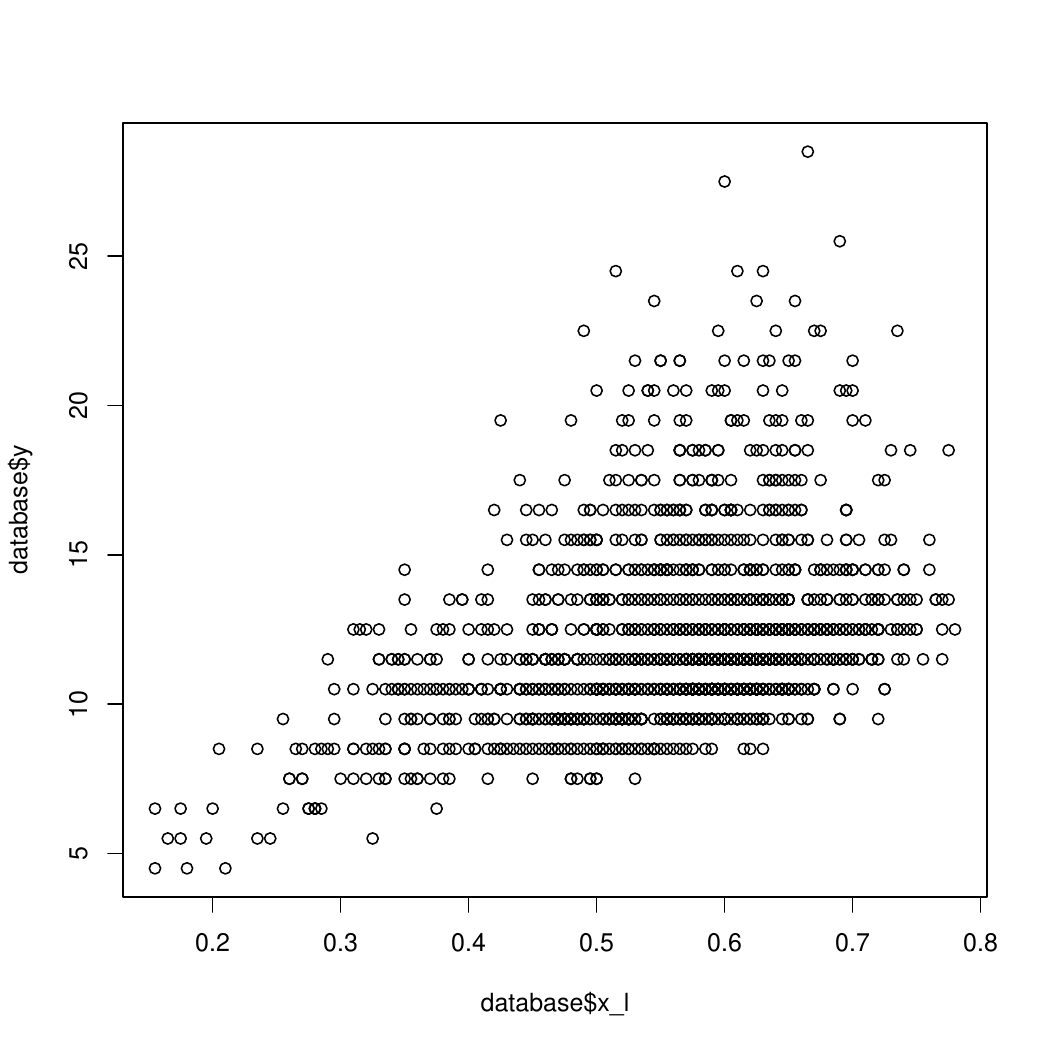
\includegraphics[width=0.45\textwidth]{male/length-1.png}
  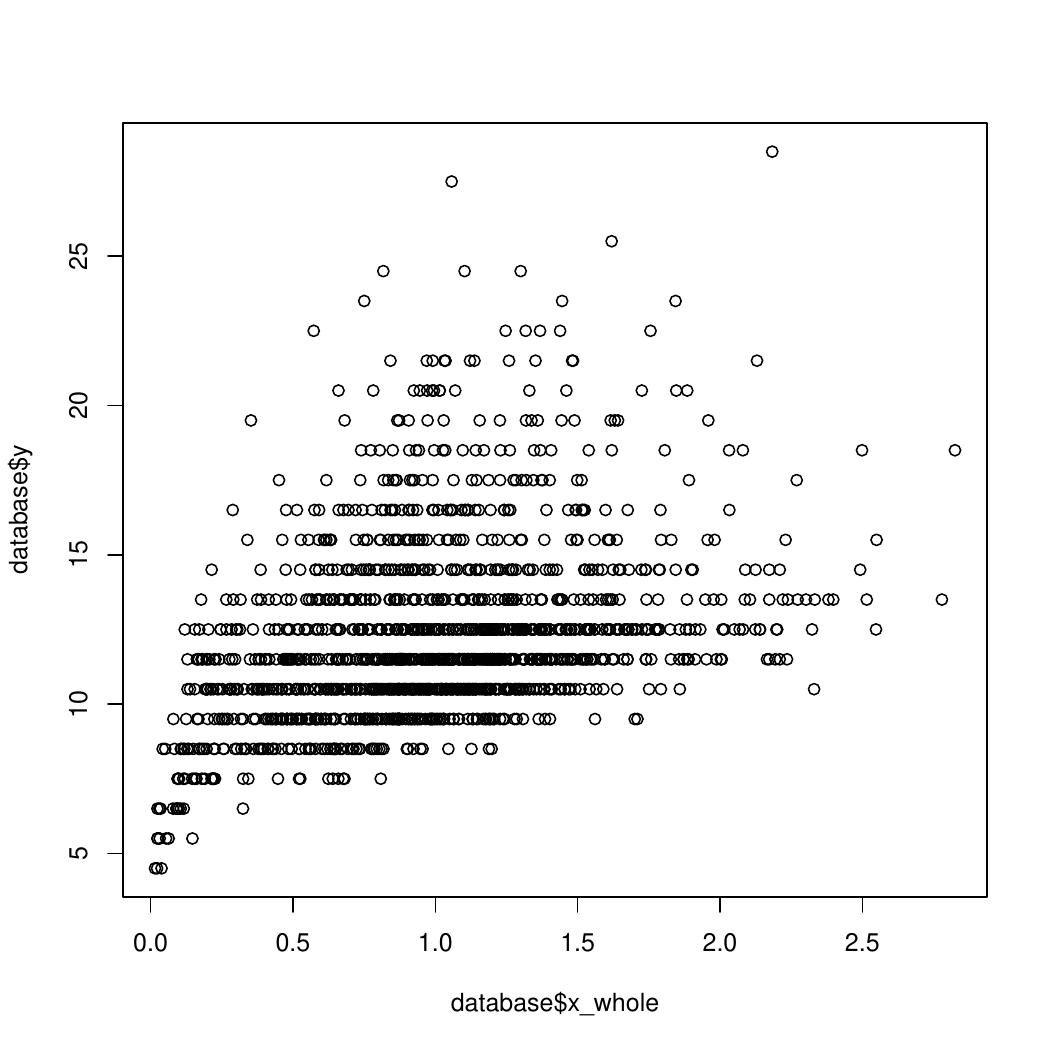
\includegraphics[width=0.45\textwidth]{male/whole_weight-1.png}
  \caption{鲍鱼的年龄与鲍鱼的长度、整体质量的关系}
\end{figure}

从图中可以看出鲍鱼的年龄与其各项参数之间具有一些线性关系。根据观测的结果,可以首先建立以下模型:

\begin{equation}
  age = \beta_0 + \beta_1 x_l + \beta_2 x_d + \beta_3 x_h + \beta_4 x_{whole} + \beta_5 x_{shucked} + \beta_6 x_{viscera} + \beta_7 x_{shell}
\end{equation}

接着我们使用回归分析的工具来进行回归分析。

\subsection{回归分析}

本文直接使用 R 语言来进行回归分析,在输入完毕数据之后直接使用 lm 函数来进行线性拟合。

\begin{minted}{r}
lm.sol <- lm(y ~ x_l + x_d + x_h + x_whole + x_shucked + x_viscera + x_shell,
  data = database)
summary(lm.sol)
\end{minted}

可以看到有以下的结果:

\begin{minted}{text}
Call:
lm(formula = y ~ x_l + x_d + x_h + x_whole + x_shucked + x_viscera + 
    x_shell, data = database)

Residuals:
    Min      1Q  Median      3Q     Max 
-8.4766 -1.4687 -0.3052  0.9788 11.6339 

Coefficients:
            Estimate Std. Error t value Pr(>|t|)    
(Intercept)   6.6924     0.5664  11.816  < 2e-16 ***
x_l          -0.4297     3.1763  -0.135    0.892    
x_d           5.0545     3.8097   1.327    0.185    
x_h          14.9002     3.4121   4.367 1.35e-05 ***
x_whole       8.6694     1.1367   7.627 4.21e-14 ***
x_shucked   -18.7931     1.2599 -14.916  < 2e-16 ***
x_viscera   -10.1695     2.0001  -5.085 4.14e-07 ***
x_shell      10.6795     1.7809   5.997 2.51e-09 ***
---
Signif. codes:  0 ‘***’ 0.001 ‘**’ 0.01 ‘*’ 0.05 ‘.’ 0.1 ‘ ’ 1

Residual standard error: 2.271 on 1520 degrees of freedom
Multiple R-squared:  0.4396,	Adjusted R-squared:  0.4371 
F-statistic: 170.4 on 7 and 1520 DF,  p-value: < 2.2e-16
\end{minted}

从上面的输出可以明显看出,鲍鱼的长度和直径的 t 检验均不明显,因此使用 step 函数进行继续分析

\begin{minted}{r}
tstep <- step(lm.sol)
summary(tstep)
\end{minted}

经过 step 函数的分析,可以看到有以下的结果:

\begin{minted}{text}
Start:  AIC=2514.08
y ~ x_l + x_d + x_h + x_whole + x_shucked + x_viscera + x_shell

            Df Sum of Sq    RSS    AIC
- x_l        1      0.09 7836.9 2512.1
- x_d        1      9.08 7845.8 2513.8
<none>                   7836.8 2514.1
- x_h        1     98.32 7935.1 2531.1
- x_viscera  1    133.29 7970.1 2537.8
- x_shell    1    185.41 8022.2 2547.8
- x_whole    1    299.92 8136.7 2569.5
- x_shucked  1   1147.15 8983.9 2720.8

Step:  AIC=2512.09
y ~ x_d + x_h + x_whole + x_shucked + x_viscera + x_shell

            Df Sum of Sq    RSS    AIC
<none>                   7836.9 2512.1
- x_d        1     33.29 7870.1 2516.6
- x_h        1     98.33 7935.2 2529.2
- x_viscera  1    135.67 7972.5 2536.3
- x_shell    1    186.25 8023.1 2546.0
- x_whole    1    299.82 8136.7 2567.5
- x_shucked  1   1155.86 8992.7 2720.3

Call:
lm(formula = y ~ x_d + x_h + x_whole + x_shucked + x_viscera + 
    x_shell, data = database)

Residuals:
    Min      1Q  Median      3Q     Max 
-8.4727 -1.4669 -0.3077  0.9777 11.6402 

Coefficients:
            Estimate Std. Error t value Pr(>|t|)    
(Intercept)   6.6616     0.5186  12.847  < 2e-16 ***
x_d           4.6011     1.8102   2.542   0.0111 *  
x_h          14.9013     3.4110   4.369 1.33e-05 ***
x_whole       8.6668     1.1361   7.628 4.17e-14 ***
x_shucked   -18.8064     1.2556 -14.978  < 2e-16 ***
x_viscera   -10.1989     1.9876  -5.131 3.25e-07 ***
x_shell      10.6912     1.7782   6.012 2.29e-09 ***
---
Signif. codes:  0 ‘***’ 0.001 ‘**’ 0.01 ‘*’ 0.05 ‘.’ 0.1 ‘ ’ 1

Residual standard error: 2.27 on 1521 degrees of freedom
Multiple R-squared:  0.4396,	Adjusted R-squared:  0.4374 
F-statistic: 198.9 on 6 and 1521 DF,  p-value: < 2.2e-16
\end{minted}

根据 step 函数的输出可以看出,删去了鲍鱼的长度变量之后,其余的各项参数均具有一定的显著性。
因此根据回归分析的结果我们可以得到一个可以用来近似估计鲍鱼的年龄的公式

\begin{equation}
  \begin{aligned}
    age =\quad & 6.6616 + 4.6011 x_d + 14.9013 x_h + 8.6668 x_{whole}  \\
    &-18.8064 x_{shucked} -10.1989 x_{viscera} + 10.6912 x_{shell}
  \end{aligned}
\end{equation}

这个公式的 t 检验和 f 检验均通过,因此这个公式可以用于性别为 $M$ 的鲍鱼的年龄估计。

\subsection{最终结果}

经过对于其他两种性别的具体分析,最终我们可以得到如下的结果:

\begin{itemize}
\item 对于性别为 M 的鲍鱼,满足

\begin{equation}
  \begin{aligned}
    age =\quad & 6.6616 + 4.6011 x_d + 14.9013 x_h + 8.6668 x_{whole}  \\
    &-18.8064 x_{shucked} -10.1989 x_{viscera} + 10.6912 x_{shell}
  \end{aligned}
\end{equation}

\item 对于性别为 F 的鲍鱼,满足

\begin{equation}
  \begin{aligned}
    age =\quad & 9.5588 -8.6322 x_l + 12.3889 x_d + 3.7143 x_h + 10.6662 x_{whole}  \\
    &-21.2263 x_{shucked} -8.8012 x_{viscera} + 7.2433 x_{shell}
  \end{aligned}
\end{equation}

\item 对于性别为 I 的鲍鱼,满足

\begin{equation}
  \begin{aligned}
    age =\quad & 4.3214 +2.8837 x_d + 28.5060 x_h + 8.2473 x_{whole}  \\
    &-14.7666 x_{shucked} -11.4193 x_{viscera} + 10.6341 x_{shell}
  \end{aligned}
\end{equation}

\end{itemize}

其中,性别为 F 的鲍鱼的年龄估计公式中不需要去除鲍鱼的长度参数,而性别为 M 和 I 的鲍鱼的年龄估计公式中需要去除鲍鱼的长度参数。

\section{其他结果}

在研究的同时发现,如果换用不同的参数和样本集进行分析,我们可以得到一些其他有趣的结果。

\subsection{忽略性别参数}

例如我们将所有样本集放到一起进行分析,即忽略鲍鱼的性别,我们可以得到如下的年龄估算公式:

\begin{equation}
  \begin{aligned}
    age =\quad & 4.3955 + 11.6337 x_d + 11.7899 x_h +  9.2562 x_{whole}  \\
    &-20.2711 x_{shucked} -9.9313 x_{viscera} + 8.6062 x_{shell}
  \end{aligned}
\end{equation}

这个估算公式的各项参数的显著性都非常高,因此也许这个公式会比按照性别分类之后分析出来的结果更有参考意义。

\subsection{忽略难以测量的参数}

另外,考虑到现实生活中的情况,我们几乎不可能将一直鲍鱼的各个不同部位的质量都拿来作为参数。
因此如果我们将参数限定为长度、直径、高度、整体质量等这些容易测量的参数中,我们可以又得到如下的年龄估算公式:

\begin{equation}
  age = 4.3365 - 11.9327 x_l + 25.7661 x_d + 20.3582 x_h
\end{equation}

该公式中的各项参数均显著,并且可以发现这个公式比前几个公式更加具有实用意义,也更加简单好求。

\newpage

\bibliographystyle{plain}

\begin{thebibliography}{99}
\bibitem{a} xxx
\end{thebibliography}

\newpage

\appendix

\section{数据集说明}

本文所采用的数据集由加州大学海湾分校网站提供,下载地址为 \url{https://archive.ics.uci.edu/ml/datasets/Abalone}。

\section{源代码一览}

\begin{minted}{r}
# 数据部分都由脚本自动生成
database <- data.frame(
  x_l = c(...),
  x_d = c(...),
  x_h = c(...),

  x_whole = c(...),
  x_shucked = c(...),
  x_viscera = c(...),
  x_shell = c(...),

  y = c(...)
)

lm.sol <- lm(y ~ x_l + x_d + x_h + x_whole + x_shucked + x_viscera + x_shell,
  data = database)
summary(lm.sol)

tstep <- step(lm.sol)
summary(tstep)

lm.sol <- lm(y ~ x_l + x_d + x_h + x_whole, data = database)
summary(lm.sol)

tstep <- step(lm.sol)
summary(tstep)
\end{minted}

\end{document}
